\begin{appendices}
\chapter{}
\vspace{-20pt}

Here, we present additional material that may answer some questions that the reader might have when reading the main text.

\paragraph{$\ell_{2}$ vs $\ell_{\infty}$ norm}: Why not use $\ell_{2}$ norm instead of $\ell_{\infty}$ norm to report the quantitative results in Figure~\ref{fig:hcp_scatter} or Figure~\ref{fig:dgw_scatter}? The reason is that the $\ell_{2}$ norm will average across the sensors. If one sensor is badly corrupted, then this would not be obvious with the $\ell_{2}$ norm because the average in the $\ell_{2}$ norm computation conceals the isolated problematic sensors with large artifacts. However, as the $\ell_\infty$ norm captures the worst sensor, it can be used to visualize pathological cases where even one sensor is corrupted. In Figure~\ref{fig:l2_norm}, we reproduce Figure~\ref{fig:hcp_scatter} using the $\ell_2$ norm instead of $\ell_{\infty}$. We can observe that, although the pattern remains the same, it is much less clear where one method outperforms the other. Even where \emph{autoreject} isn't performing as well, it is not  visible due to the averaging % effect.

\begin{figure}[htb]
	\centering
	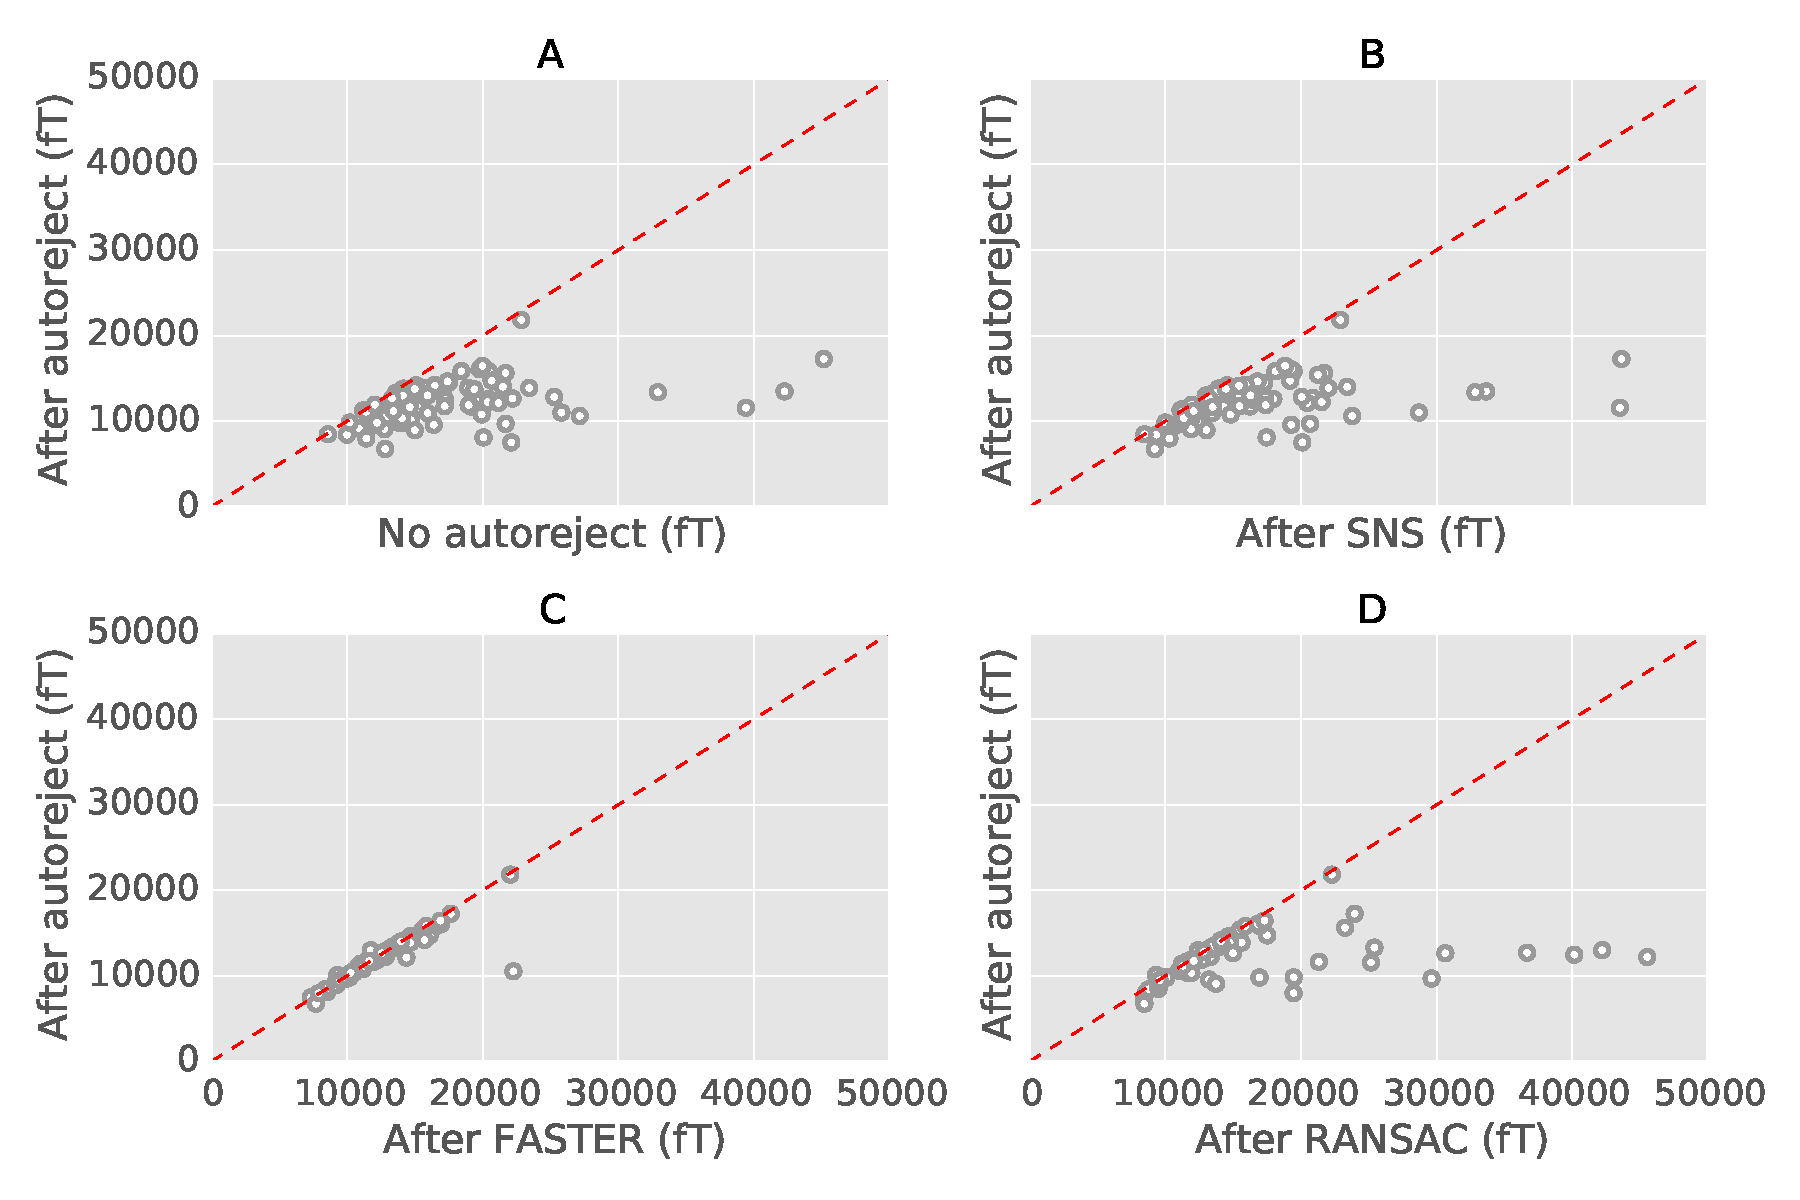
\includegraphics[width=0.8\linewidth]{figures/figure4_supp.pdf}
    \caption{Scatter plots for the results with the HCP data. This figure uses the same data as in Figure~\ref{fig:hcp_scatter} from the main text, but with  $\|\cdot\|_2$ norm instead of the $\|\cdot\|_\infty$ norm for computing the difference between the HCP ground truth and the method. As before, each circle is a subject. (A) \textit{autoreject (local)} against no rejection, (B) \textit{autoreject (local)} against Sensor Noise Suppression (SNS) (SNS), (C) \textit{autoreject} against FASTER, (D) \textit{autoreject (local)} against RANSAC. Data points below the dotted red line indicate subjects for which \textit{autoreject (local)} outperforms the alternative method.}
    \label{fig:l2_norm}
\end{figure}

\chapter{}
\vspace{-20pt}

\section{Details of the E-Step}

%\umut{I will put more derivations here.}

Computing the weights that are required in the M-step requires us to compute the expectation of $\frac1{\phi_{n,t}}$ under the posterior distribution $p(\phi_{n,t}|x,d,z)$, which is not analytically available. 

Monte Carlo methods are numerical techniques that can be used to approximately compute the expectations of the form:
\begin{align}
\mathds{E}[f(\phi_{n,t})] = \int f(\phi_{n,t}) \pi(\phi_{n,t}) d\phi_{n,t} \approx \frac1{J} \sum_{j=1}^J f(\phi_{n,t}^{(j)}) \label{eqn:mc}
\end{align}
where $\phi_{n,t}^{(j)}$ are some samples drawn from $\pi(\phi_{n,t}) \triangleq p(\phi_{n,t}|x,d,z)$ and $f(\phi) = 1/\phi$ in our case. However, in our case, sampling directly from $\pi(\phi_{n,t})$ is also unfortunately intractable.

%  through a transition kernel;  $ \mathbf{\Theta}^{(i+1)} \sim {\cal T}(\mathbf{\Theta}|\mathbf{\Theta}^{(i)})$

MCMC methods generate samples from the target distribution $\pi(\phi_{n,t})$ by forming a Markov chain, whose stationary distribution is $\pi(\phi_{n,t})$, 
%
so that $\pi(\phi_{n,t}) = \int {\cal T}(\phi_{n,t}|\phi_{n,t}') p(\phi_{n,t}') d\phi_{n,t}'$, where ${\cal T}$ denotes the transition kernel of the Markov chain. 

In this study, we develop a Metropolis-Hastings (MH) algorithm, that implicitly forms a transition kernel. 
%
The MH algorithm generates samples from a target distribution $\pi(\phi_{n,t})$ in two steps. First, it generates a random sample $\phi_{n,t}'$ from a \emph{proposal} distribution $\phi_{n,t}' \sim q(\phi_{n,t}'|\phi_{n,t}^{(j)})$, then computes an acceptance probability $\text{acc}(\phi_{n,t}^{(j)} \rightarrow \phi_{n,t}')$ and draws a uniform random number $u \sim {\cal U}([0, 1])$. If $u < \text{acc}(\phi_{n,t}^{(j)} \rightarrow \phi_{n,t}')$, it accepts the sample and sets $\phi_{n,t}^{(j+1)} = \phi_{n,t}'$; otherwise it rejects the sample and sets $\phi_{n,t}^{(j+1)} = \phi_{n,t}^{(j)}$. The acceptance probability is given as follows
\begin{align}
\text{acc}(\phi_{n,t} \rightarrow \phi_{n,t}') = \min \Bigr\{1, \frac{q(\phi_{n,t}|\phi_{n,t}') \pi(\phi_{n,t}')}{q(\phi_{n,t}'|\phi_{n,t}) \pi(\phi_{n,t})}\Bigr\} = \min \Bigr\{1, \frac{q(\phi_{n,t}|\phi_{n,t}') p(x_{n,t}|\phi_{n,t}',d,z) p(\phi_{n,t}') }{q(\phi_{n,t}'|\phi_{n,t}) p(x_{n,t}|\phi_{n,t},d,z) p(\phi_{n,t}) }\Bigr\}
\end{align}
where the last equality is obtained by applying the Bayes rule on $\pi$. 

The acceptance probability requires the prior distribution of $\phi$ to be evaluated. Unfortunately, this is intractable in our case since this prior distribution is chosen to be a positive $\alpha$-stable distribution whose PDF does not have an analytical form. As a remedy, we choose the prior distribution of $\phi_{n,t}$ as the proposal distribution, such $q(\phi_{n,t}|\phi_{n,t}') = p(\phi_{n,t})$. This enables us to simplify the acceptance probability. Accordingly, for each $\phi_{n,t}$, we have the following acceptance probability:
\begin{align}
  \text{acc}(\phi_{n,t}^{(i,j)} \rightarrow \phi_{n,t}' ) \triangleq \min  \Bigl\{1, \exp(\log \phi_{n,t}^{(i,j)} - \log \phi_{n,t}')/2 + (x_{n,t} - \hat{x}^{(i)}_{n,t})^2 (1/{\phi_{n,t}^{(i,j)}} - 1/{\phi_{n,t}'}) \Bigr\}.
\end{align}
Thanks to the simplification, this probability is tractable and can be easily computed. 

\section{Details of the M-Step}

\subsection{Solving for the activations}
In the M-step, we optimize~\eqref{eq:problem_definition_z} to find the activations $z_n^{(i)}$ of each trial $n$ independently. To keep the notation simple, we will drop the index for the iteration number $i$ of the EM algorithm.

First, this equation can be rewritten by concatenating the Toeplitz matrices for the $K$ atoms into a big matrix $D = [D^1, D^2, ..., D^K] \in \bbR^{T \times KT}$ and the activations for different atoms into a single vector $\bar{z}_n = [(\bar{z}_n^1)^\top, (\bar{z}_n^2)^\top, ..., (\bar{z}_n^K)^\top]^\top \in \bbR^{KT}_+$ where $(\cdot)^\top$ denotes the transposition operation. Recall that $\bar{z}_n^k$ is a zero-padded version of $z_n^k$. This leads to a simpler formulation and the objective function $\mathcal{L}(d, z)$:
\begin{equation}
\mathcal{L}(d, z) = \sum_{n=1}^{N} \frac{1}{2}\|\sqrt{w_{n}} \odot (x_{n} - D \bar{z}_{n})\|_{2}^{2} + \lambda \mathbbm{1}^\top \bar{z}_{n} \enspace ,
\label{eq:problem_definition_d_simple}
\end{equation}
where $\mathbbm{1} \in \bbR^{KT}$ is a vector of ones.

The derivative w.r.t. $z_n$ now reads:
\begin{equation}
\frac{\partial \mathcal{L}(d, z)}{\partial \bar{z}_n}
= D^\top(w_n \odot (x_n - D\bar{z}_n)) + \lambda \mathbbm{1}^\top \enspace .
\end{equation}
In practice, this big matrix $D$ is never assembled and all operations are carried out using convolutions. Note also that we do not update the zeros from the padding in $\bar{z}_n^k$. Now that we have the gradient, the activations can be estimated using a efficient quasi-Newton solver such as L-BFGS-B, taking into account the box posititivy constraint $0 \leq z_n \leq \infty$.
%In the case of PG algorithm, one has a modified soft thresholding operator given by a rectified linear function $\mathcal{S}_{\lambda t}=\mathrm{max}(0, z_i - \lambda t)$.
%The step size for ISTA and FISTA can be chosen to be the inverse of the Lipschitz constant which is equal to the largest eigenvalue of $D^{\top}(\tau_{i} \odot D)$. In practice, this is estimated using the power iteration method \mainak{[ref]} with warm restarts.

For each trial, one iteration costs $\mathcal{O}(LKT)$.

\subsection{Solving for the atoms}

In the M-step, we optimize \eqref{eq:problem_definition_d} to find the atoms $d^k$.
As when solving for the activations $z_n$, we can remove the summation over the atoms by concatenating the delayed matrices into $Z_{n}=[Z_{n}^1, Z_{n}^2, \dots, Z_{n}^K] \in \bbR^{T \times KL}$ and $d=[(d^1)^\top, (d^2)^\top, ..., (d^K)^\top]^\top \in \bbR^{KL}$. This leads to the simpler formulation:
%
\begin{align}
& \min_{d} \sum_{n=1}^{N} \frac{1}{2}\|\sqrt{w_n} \odot (x_{n} - Z_{n}d)\|_{2}^{2}, \quad \text{  s.t.  } \|d^k\|_2^2 \leq 1 \enspace.
\label{eq:subproblem_d}
\end{align}
%
%If not for the constraint, this is a classic least square problem which has a known closed-form solution:
%\begin{equation}
%\hat{d} = \Big(\sum_{i=1}^N Z_i^{\top}(\tau_{i} \odot Z_i) \Big)^{-1}\sum_{i=1}^{N} (\tau_{i} \odot Z_i)^{\top}x_i
%\end{equation}
%\ag{say somewhere that FFT based cross-correlation is not possible anymore with EM sample weights}
%\ag{we need to keep the maths for what we are doing and put all the rest in appendix. No need to remind text book notions of optim in main text.}
%
 The Lagrangian of this problem is given by:
%
\begin{equation}
g(d, \beta) = \sum_{n=1}^{N} \frac{1}{2}\|\sqrt{w_n} \odot (x_{n} - \sum_{k=1}^{K} Z_{n}^{k}d^{k}) \|_{2}^{2} + \sum_k \beta^k (\|d^k\|_2^{2} - 1) \quad \text{s.t. } \beta^k \geq 0 \enspace,
\end{equation}
%
where $\beta = (\beta^1, \beta^2, ..., \beta^K)$ are the dual variables. Therefore, the dual problem is:
%
\begin{align}
\min_{d}{g(d, \beta)} = g(d^{*}, \beta)
\end{align}
%
where $d^*$, the primal optimal, is given by:
%
\begin{equation}
d^{*} = (\sum_{n=1}^N Z_n^{\top}(w_{n} \odot Z_n) + \bar{\beta} )^{-1}\sum_{n=1}^{N}(w_{n} \odot Z_n)^{\top}x_n
\label{eq:dual_optimal}
\end{equation}
%
with $\bar{\beta} = \mathrm{diag}([\mathbbm{1}\beta^1, \mathbbm{1}\beta^2, ..., \mathbbm{1}\beta^K]) \in \bbR^{KL}$ with $\mathbbm{1} \in \bbR^{L}$. The gradient for the dual variable $\beta^k$ is given by:
%
\begin{equation}
\frac{\partial g(d^{*}, \beta)}{\partial \beta^k}  = \|{d^{*}}^k\|_2^2 - 1,
\end{equation}
%
with ${d^{*}}^k$ computed from~\eqref{eq:dual_optimal}.
%Of course, we do not know the primal optimal $\hat{d}^k$ offhand, as it is what we want to estimate.
We can solve this iteratively using again L-BFGS-B taking into account the positivity constraint $\beta^k \geq 0$ for all $k$.
% It amounts to computing the primal update at each step, then the dual gradients according to the updated primal, then updating the dual using the gradient and continuing this way until convergence. \mainak{Is there a name for this class of algorithms, so the reader can easily relate?}
What we have described so far solves for all the atoms simultaneously. However, it is also possible to estimate the atoms sequentially one at a time using a block coordinate descent (BCD) approach, as in the work of \citep{mairal2010online}. In each iteration of the BCD algorithm, a residual $r_n^k$ is computed as given by:
%
\begin{equation}
r_n^k = x_n - \sum_{k'\neq k} Z^{k'}_{n}d^{k'}
\end{equation}
%
and correspondingly subproblem \ref{eq:subproblem_d} becomes:
%
\begin{align}
& \min_{d^k} \sum_{n=1}^{N} \frac{1}{2}\|\sqrt{w_n} \odot (r^k_{n} - Z^k_{n}d^k)\|_{2}^{2}, \quad \text{  s.t.  } \|d^k\|_2^2 \leq 1, \enspace.
\label{eq:subproblem_d_block}
\end{align}
%
%Solving for atoms can be done all atoms simultaneously or using a block coordinate descent approach by looping sequentially over atoms.
which is solved in the same way as subproblem~\ref{eq:subproblem_d}. Now, in the simultaneous case, we construct one linear problem in $\mathcal{O}(L^2K^2TN)$ and one iteration costs $\mathcal{O}(L^3K^3)$. However, in the BCD strategy, we construct $K$ linear problems in $\mathcal{O}(L^2TN)$ and one iteration costs only $\mathcal{O}(L^3)$.
Interestingly, when the weights $w_n$ are all identical, we can 
use the fact that for one atom $k$, the matrix $\sum_{i=1}^{N}(Z_i^k)^T Z_i^k$ is Toeplitz. In this case, we can construct $K$ linear problems in only $\mathcal{O}(LTN)$ and one iteration costs only $\mathcal{O}(L^2)$.

For the benefit of the reader, we summarize the complexity of the M-step in Table~\ref{table:complexity_m}. We note $p$ and $q$ the number of iterations in the L-BFGS-B methods for the activations update and atoms update.


% \subsection{Computational tricks and complexity analysis}
\begin{table}[htb]
\begin{center}
\begin{tabular}{|l|l|}
\hline
Method & Complexity \\
\hline
Solving activations $z$ & $p\min(L, \log(T))KTN$ \\
%\hline
%z update LBFGS-B & $\min(pLKTN, p\log(T)KTN)$ \\
%\hline
%d update primal & $L^2K^2TN + qL^2K^2$ \\
%\hline
Solving atoms $d$ & $L^2K^2TN + qL^3K^3$ \\
%\hline
%d update block primal & $LKTN + qL^2K$ \\
%\hline
Solving atoms $d$ (sequential) & $LKTN + qL^2K$ \\
\hline
\end{tabular}
\vspace{5pt}
\caption{Complexity analysis of the M-step, where $p$ and $q$ are the number of iterations in the L-BFGS-B solvers for the activations and atoms updates.}
\label{table:complexity_m}
\end{center}
\end{table}

\section{Additional Experiments: M-step speed benchmark}

\subsection{Comparison with state of the art}

\begin{figure}[htb]
    \centering
     \subfigure[$K=2$, $L=32$.]{
     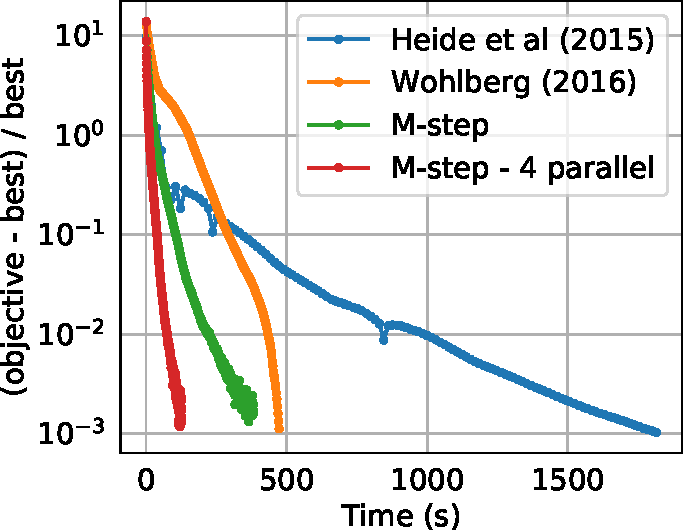
\includegraphics[width=0.31\linewidth]{figures/relative_2_32.pdf}}
     \subfigure[$K=2$, $L=128$.]{
     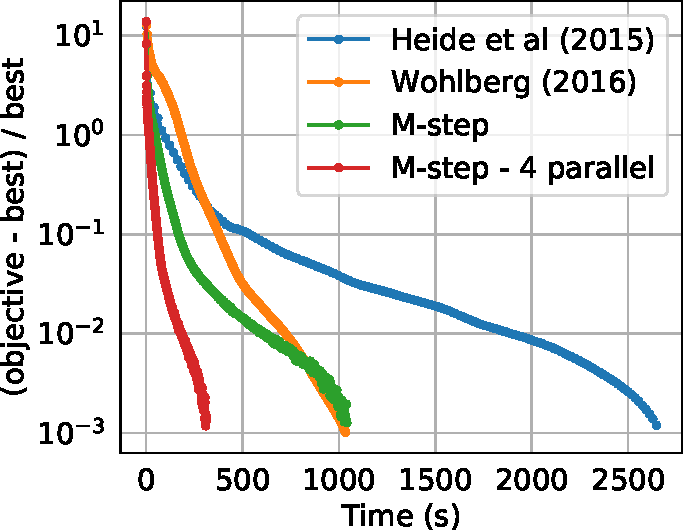
\includegraphics[width=0.31\textwidth]{figures/relative_2_128.pdf}}
     \subfigure[$K=10$, $L=32$.]{
     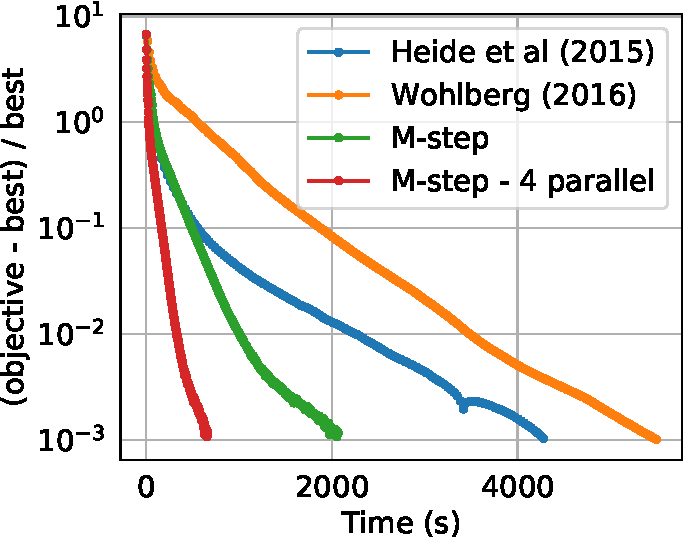
\includegraphics[width=0.31\textwidth]{figures/relative_10_32.pdf}}
    \vspace{-5pt}
    \caption{Convergence speed of the relative objective function. The y-axis shows the objective function relative to the obtained minimum for each run: $(f(x) - f(x^*))/f(x^*)$. Each curve is the geometrical mean over 24 different random initializations.}
    \label{fig:convergence_setups}
\end{figure}

Here, we compare convergence plots of our algorithm against a number of state-of-art methods. The details of the experimental setup are described in Section~\ref{sec:experiments}. Fig.~\ref{fig:convergence_setups} demonstrates on a variety of setups the computational
advantage of our quasi-Newton approach to solve the M-step.
Note that Fig.~\ref{fig:convergence}b is in fact a summary of Fig.~\ref{fig:convergence_setups}. 
Indeed, we can verify that ADMM methods converge quickly to a modest accuracy, but take much longer to converge to a high accuracy.\citep{boyd2011distributed}

Next, in Fig.~\ref{fig:convergence_traditional}, we show more traditional convergence plots. In contrast to Fig.~\ref{fig:convergence} or \ref{fig:convergence_setups} where the relative objective function is shown, here we plot the absolute value of the objective function. We can now verify that each of the methods have indeed converged to their respective local minimum. Of course, owing to the non-convex nature of the problem, they do not necessarily converge to the same local minimum.
\begin{figure}[htb]
    \centering
     \subfigure[$K=2$, $L=32$.]{
     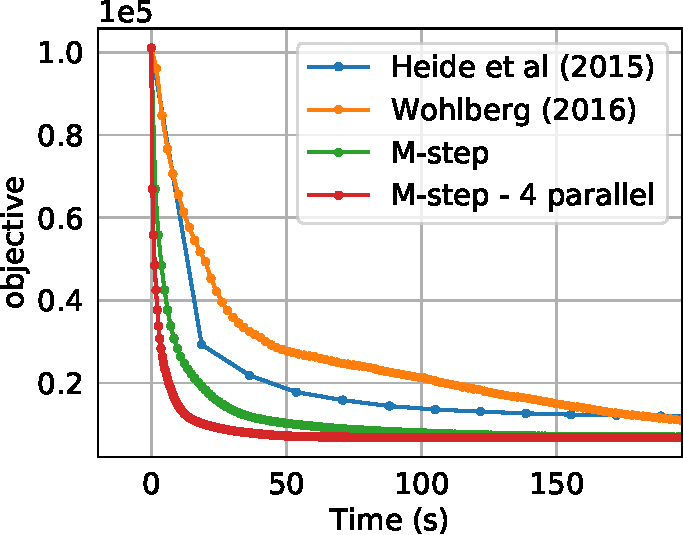
\includegraphics[width=0.31\linewidth]{figures/plateau_2_32.pdf}}
     \subfigure[$K=2$, $L=128$.]{
     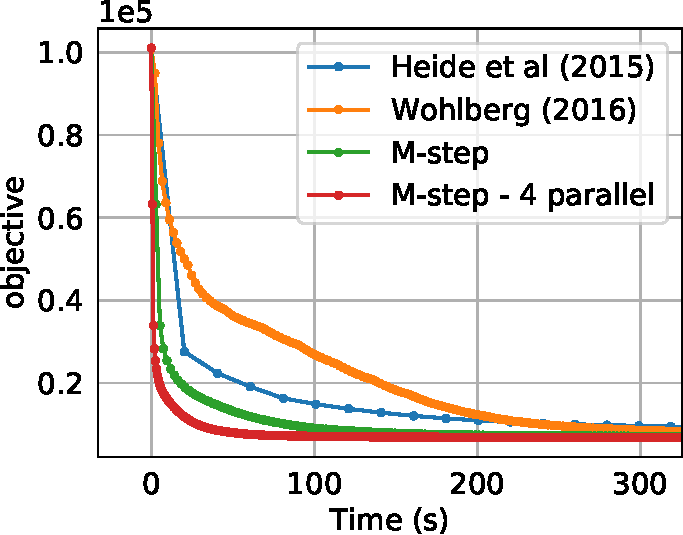
\includegraphics[width=0.31\textwidth]{figures/plateau_2_128.pdf}}
     \subfigure[$K=10$, $L=32$.]{
     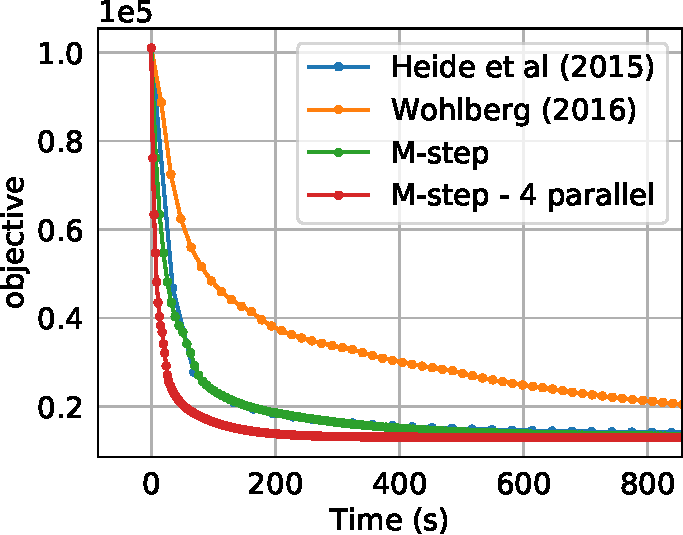
\includegraphics[width=0.31\textwidth]{figures/plateau_10_32.pdf}}
    \vspace{-5pt}
    \caption{Convergence of the objective function as a function of time. The y-axis shows the absolute objective function $f(x)$. Each curve is the mean over 24 different random initializations.}
    \label{fig:convergence_traditional}
\end{figure}

\subsection{Comparison of solver for the activations subproblem}

Finally, we compare convergence plots of our algorithm using different solvers for the $z$-update: ISTA, FISTA, and L-BFGS-B. The rationale for choosing a quasi-Newton solver for the $z$-update becomes clear in  Fig.~\ref{fig:convergence_z_update} as the L-BFGS-B solver turns out to be computationally advantageous on a variety of setups.

\begin{figure}[h]
    \centering
     \subfigure[$K=2$, $L=32$.]{
     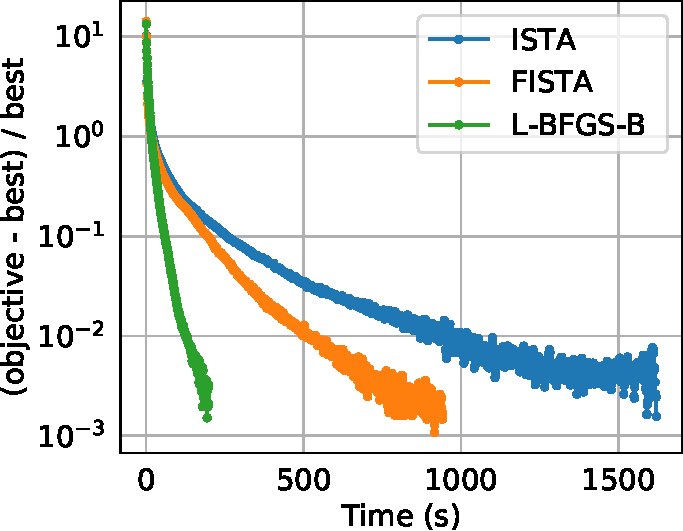
\includegraphics[width=0.31\linewidth]{figures/fista_2_32.pdf}}
     \subfigure[$K=2$, $L=128$.]{
     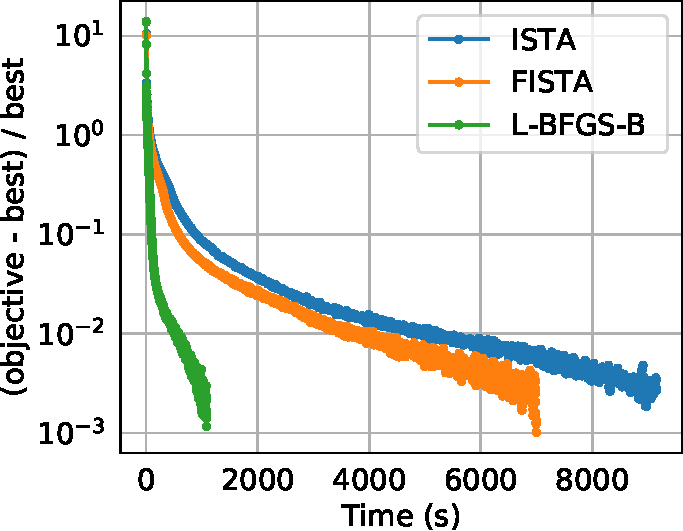
\includegraphics[width=0.31\textwidth]{figures/fista_2_128.pdf}}
     \subfigure[$K=10$, $L=32$.]{
     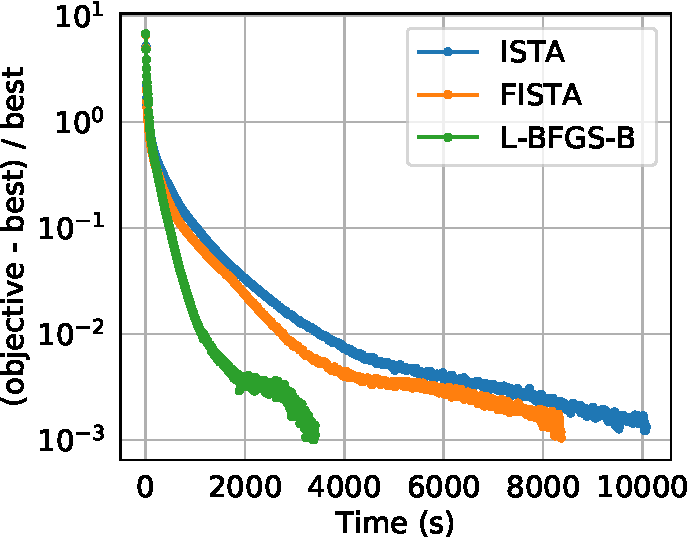
\includegraphics[width=0.31\textwidth]{figures/fista_10_32.pdf}}
    \vspace{-5pt}
    \caption{Convergence speed of the relative objective function. The y-axis shows the objective function relative to the obtained minimum for each run: $(f(x) - f(x^*))/f(x^*)$. Each curve is the geometrical mean over 24 different random initializations.}
    \label{fig:convergence_z_update}
\end{figure}

\end{appendices}